%& C:\Users\lizil\AppData\Roaming\TikzEdt\TikzEdt\023~1.0\TEMP_H~1
\begin{document}
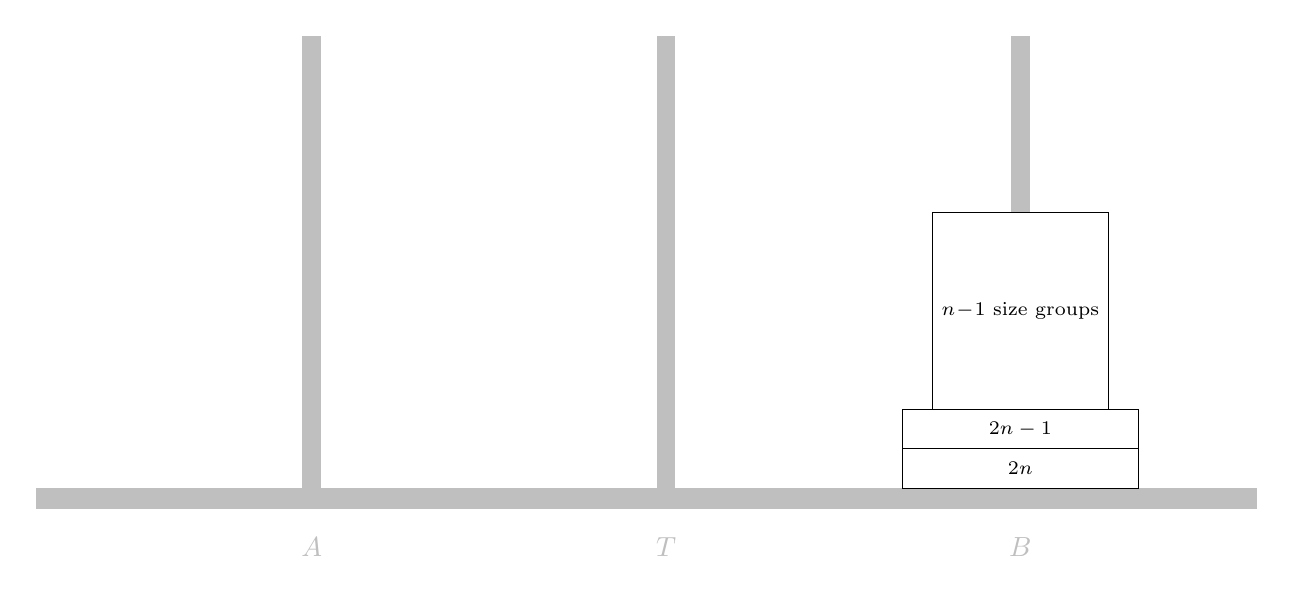
\begin{tikzpicture}
\tikzstyle{largestone} = [minimum width=3cm,minimum height=0.5cm,draw,fill=white,font=\scriptsize];
\tikzstyle{smallerpile} = [minimum width=2cm,minimum height=2.5cm,draw,text width=2cm,text centered,fill=white,font=\scriptsize];
\tikzstyle{tray} = [gray!50];
\tikzstyle{peg} = [fill=gray!50,minimum width=0.1cm,minimum height=6cm];

\filldraw[tray]   (-7.5,0) rectangle (8,0.25);
\node[tray] at (-4,-0.5) {$A$};
\node [tray] at (0.5,-0.5) {$T$};
\node [tray] at (5,-0.5) {$B$};
\node [peg] at (-4,3) {};
\node [peg] at (0.5,3) {};
\node [peg] at (5,3) {};

\node [largestone] at (5,0.5) {$2n$};
\node [largestone] at (5,1) {$2n-1$};
\node [smallerpile] at (5,2.5) {$n-1$ size groups};


\usetikzlibrary{calc}
\pgftransformreset
\node[inner sep=0pt,outer sep=0pt,minimum size=0pt,line width=0pt,text width=0pt,text height=0pt] at (current bounding box) {};
%add border to avoid cropping by pdflibnet
\foreach \border in {0.1}
  \useasboundingbox (current bounding box.south west)+(-\border,-\border) rectangle (current bounding box.north east)+(\border,\border);
\newwrite\metadatafile
\immediate\openout\metadatafile=\jobname_BB.txt
\path
  let
    \p1=(current bounding box.south west),
    \p2=(current bounding box.north east)
  in
  node[inner sep=0pt,outer sep=0pt,minimum size=0pt,line width=0pt,text width=0pt,text height=0pt,draw=white] at (current bounding box) {
\immediate\write\metadatafile{\p1,\p2}
};
\immediate\closeout\metadatafile
\end{tikzpicture}

\end{document}
